\documentclass[10pt]{beamer}
\usetheme{default}
\setbeamercovered{invisible}
\setbeamertemplate{navigation symbols}{}
\setbeamertemplate{footline}{
    \flushright{\hfill \insertframenumber{}/\inserttotalframenumber}
}

\usepackage{listings}

% User-defined colors.
\definecolor{DarkGreen}{rgb}{0, .5, 0}
\definecolor{DarkBlue}{rgb}{0, 0, .5}
\definecolor{DarkRed}{rgb}{.5, 0, 0}
\definecolor{LightGray}{rgb}{.95, .95, .95}
\definecolor{White}{rgb}{1.0,1.0,1.0}
\definecolor{darkblue}{rgb}{0,0,0.9}
\definecolor{darkred}{rgb}{0.8,0,0}
\definecolor{darkgreen}{rgb}{0.0,0.85,0}

% Settings for listing class.
\lstset{
  language=C++,                        % The default language
  basicstyle=\small\ttfamily,          % The basic style
  backgroundcolor=\color{White},       % Set listing background
  keywordstyle=\color{DarkBlue}\bfseries, % Set keyword style
  commentstyle=\color{DarkGreen}\itshape, % Set comment style
  stringstyle=\color{DarkRed}, % Set string constant style
  extendedchars=true % Allow extended characters
  breaklines=true,
  basewidth={0.5em,0.4em},
  fontadjust=true,
  linewidth=\textwidth,
  breakatwhitespace=true,
  showstringspaces=false,
  lineskip=0ex, %  frame=single
}

\begin{document}
    \title{Optimization, debugging and profiling}
    \author{Pasquale Claudio Africa}
    \date{07/05/2020}

\begin{frame}[plain, noframenumbering]
    \maketitle
\end{frame}

\begin{frame}{CPU vs. RAM}
    \begin{figure}
        \centering
        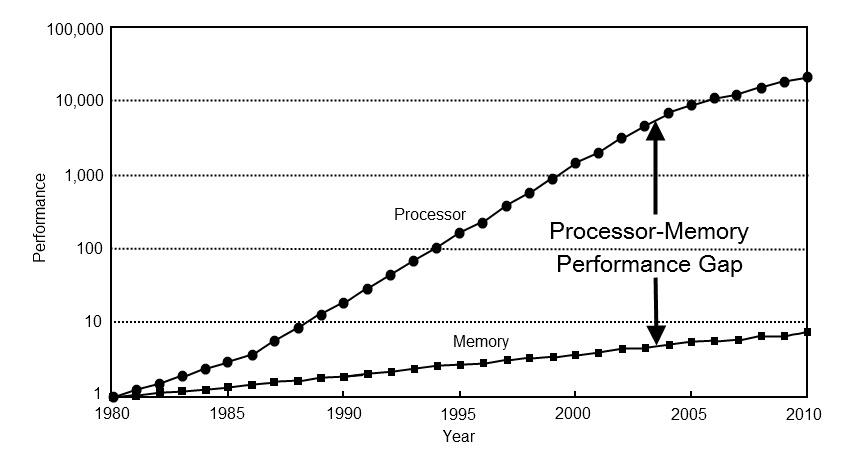
\includegraphics[width=\textwidth]{images/cpu_memory_performance_gap.png}
        \caption{\textit{Computer Architecture: A Quantitative Approach by John L. Hennessy, David A. Patterson, Andrea C. Arpaci-Dusseau}}
    \end{figure}
\end{frame}

\begin{frame}{Memory layout}
    \begin{figure}
        \centering
        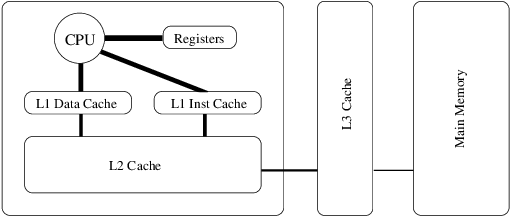
\includegraphics[width=\textwidth]{images/memory_layout.png}
        \caption{Typical memory layout of a computer.}
    \end{figure}
\end{frame}

\begin{frame}{Exercise 1: how memory access affects performance}
    This exercise is inspired by \href{https://bitbashing.io/memory-performance.html}{\textcolor{DarkBlue}{this post}}.
    \vfill
    The source file \texttt{01-memory-access/01-base.cpp} implements a very simple algorithm, where a \texttt{std::vector} of size equal to an integer multiple of the cache memory is filled with random numbers and applied some simple mathematical operation (function \texttt{compute()}) for a specified amount of iterations.
    \vfill
    Compare the performance of the following three ways of accessing elements in the vector:
    \begin{enumerate}
        \item sequential value access;
        \item sequential pointer access;
        \item random pointer access.
    \end{enumerate}
\end{frame}

\begin{frame}{Memory layout}
    \begin{figure}
        \centering
        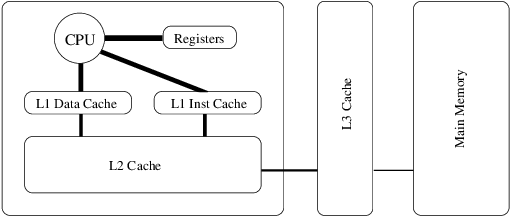
\includegraphics[width=\textwidth]{images/memory_layout.png}
        \caption{Typical memory layout of a computer.}
    \end{figure}
\end{frame}

\begin{frame}{Exercise 2 - Optimization techniques\footnote{See also: \url{https://github.com/ArtemKovera/code-optimization-techniques}}}
    \begin{enumerate}
        \item Implement a function that allocates a \texttt{std::vector} and, taking an index as an input, simply returns the corresponding value. Compare the performance with respect to declaring the vector \texttt{static}.
        \item Implement a function that multiplies all element in a \texttt{std::vector} by looping over all its elements and returns the result. Compare the performance with respect to rewriting the loop using unrolling.
        \item Optimize the memory occupation of an object of class \texttt{Class1} by properly aligning/padding the data structure.
    \end{enumerate}
\end{frame}

\begin{frame}[fragile]{Data structure alignment\footnote{See also: \url{https://www.geeksforgeeks.org/data-structure-alignment/}}}
    \begin{lstlisting}
class MyClass
{
  char a;      // 1 byte.
  short int b; // 2 bytes.
  int c;       // 4 bytes.
  char d;      // 1 bytes.
}
    \end{lstlisting}
    \begin{figure}
        \centering
        \only<1>{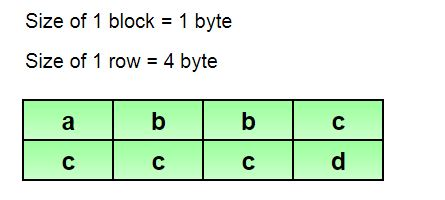
\includegraphics[width=0.75\textwidth]{images/padding_pre.jpg}}
        \only<2>{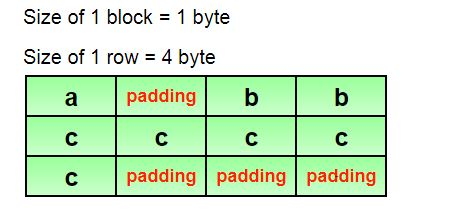
\includegraphics[width=0.75\textwidth]{images/padding_post.jpg}}
        \caption{How data is \alt<1>{\textbf{not}}{actually} stored.}
    \end{figure}
\end{frame}


\begin{frame}{Exercise 3}
Starting from the provided implementation of the class for dense matrices (and column vectors represented as 1-column matrices) based on \lstinline{std::vector}, implement the following methods:
\begin{itemize}
\item \lstinline{transpose()}: $A = A^{T}$.
\item \lstinline{operator*}: matrix-matrix and matrix-vector multiplication.
\end{itemize}
\end{frame}

\begin{frame}{Exercise 3 - What you need to know}
\begin{itemize}
\item The implemented matrix class is organized as
      \textbf{column-major}, \textit{i.e.}
      $A(i, j) = $ \lstinline{data[i + j * n_rows()]},
      conversion from 1D to 2D indexing is performed by the utility
      method \lstinline{sub2ind}.\\[3mm]
\item Access to elements is implemented both in \texttt{const} and non-\texttt{const} versions, by overloading \lstinline{operator()}. \\[3mm]
\item Data is private, \textit{getter methods} expose what is needed to the user, both \texttt{const} and non-\texttt{const} versions are provided. \\[3mm]
\item Naive implementation of matrix-matrix multiplication is slow because it has low \textit{data locality}, simply transposing the left matrix factor improves performance significantly\footnote{See also: \textit{M. Kowarschik, C. Weiß. (2002). Lecture Notes in Computer Science. 213-232. DOI: 10.1007/3-540-36574-5\_10} for further details.}.\\[3mm]
\item The \lstinline{\#include "test_matrix_mult.hpp"} header provides timing utilities, \lstinline{tic()} and \lstinline{toc(x)} macros start and stop the timer.
\end{itemize}
\end{frame}

\begin{frame}{Matrix-matrix multiplication: loop tiling}
    \begin{figure}
        \centering
        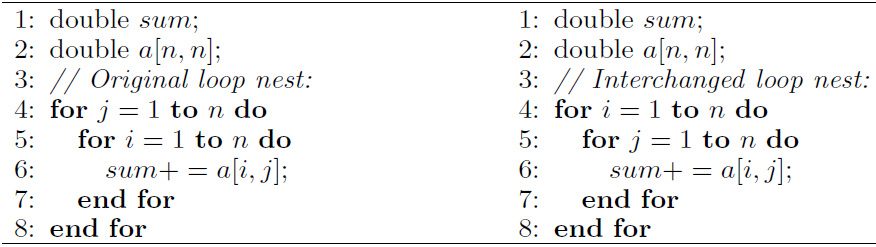
\includegraphics[width=\textwidth]{images/loop_tiling.png}
        \caption{Loop tiling.}
    \end{figure}
\end{frame}

\begin{frame}{Exercise 3.2}
    \begin{itemize}
        \item Transpose the first factor in matrix multiplication before performing the product.
        \item Compare the execution speed with respect to the previous implementation.
        \item Generate a coverage report using \texttt{lcov}.
    \end{itemize}
\end{frame}

\begin{frame}{Exercise 3.3}
    \begin{itemize}
        \item Include the \texttt{Eigen/Dense} header.
        \item Use the \texttt{Eigen::Map} template class to wrap the matrix data and interpret it as \texttt{Eigen::MatrixXd}.
        \item Compare the execution speed with respect to the previous implementations.
    \end{itemize}
\end{frame}

\begin{frame}{Exercise 4}
The program \texttt{integer-list} in the directory \texttt{02-bug} has:

\begin{itemize}
    \item a compile error;
    \item a run-time error;
    \item a memory leak;
    \item a potential memory leak that is not captured by the \texttt{main}.
\end{itemize}
\vspace{0.5cm}
Find all the issues and fix them. \\[3mm]

Get help by using \texttt{gdb} and \texttt{valgrind}.\\[3mm]

The directory \texttt{02-bug-solution} contains the fixed code,
please don't look at it before trying to solve the exercise by yourself!
\end{frame}

\end{document}
